\chapter{光学成像辅助的压缩感知缺陷检测}

\section{问题描述}

文献 \cite{XDUCLBIC} 指出,在基于压缩感知的缺陷检测系统中,太阳能电池表面
栅状电极覆盖的区域的光电转化效率为 $0$ 。这些线状区域的存在严重破坏了信号
的稀疏性。对于全变分最小化方法,求梯度完全不能降低线状目标的稀疏性;
对于 $\ell_1$ 最小化方法,必须寻找一个能够稀疏表示直线的字典,才能降低
栅状电极的稀疏性。目前确实有这样的字典存在,即\emph{脊波}(Ridgelet)
和\emph{曲波}(Curvelet)变换。\cite{ridgelet}\cite{curvelet} 十分巧合的
是,这两种变换正是由压缩感知理论的提出者 Cand\`es 和 Donoho 发明的。
然而,脊波和曲波变换的数学形式较为复杂,程序运行较慢,对于迭代次数较多的
优化问题而言,会极大增加优化算法的运行时间。

本文采用另一种方案,解决栅状电极带来的稀疏性退化问题。由于栅状电极在光学
上是可见的,我们可以用光学相机获取栅状电极的位置。从信息论的角度出发,当
我们获得了栅状电极的位置信息后,如果我们能够合理地运用这些信息,就可能
减少压缩采样过程需要获取的信息量,从而减少采样次数,提高检测效率。本章
的后续内容将表明,这的确是可行的。

\section{数学模型}

考虑问题的物理本质,栅状电极覆盖区域的光电转化效率为 $0$ ,纯粹是由于它
被电极覆盖的缘故,与电极之下的硅材料毫无关系。假如栅状电极是透明的(现实中
并没有这样良好的电极材料),它对测量结果没有影响,得到的测量结果是稀疏的。
然而,由于栅状电极的\emph{遮挡},被遮挡区域的测量值直接变为 $0$ ,导致稀疏
性退化。这样,自然想到采用\emph{图像修补}算法,去除图像上的遮挡,尽可能
恢复未被遮挡的,稀疏的图像,从而提高压缩感知的效率和准确性。

下面给出图像修补问题的数学描述:
\begin{problem}[图像修补]
设有一矩阵 $H = diag\{W\}$,$W \in \{0,1\}^{N}$。设 $x$ 是一维向量
化的图像,则被遮挡并有噪声 $z$ 污染的图像为
\begin{equation}
y = Hx + z
\end{equation}
已知 $y$ 和 $H$ ,恢复未被遮挡的图像 $x$。
\end{problem}

和压缩感知恢复问题一样,图像修补问题亦可通过求解全变分最小化或 $\ell_1$
最小化解决,下面以全变分最小化为例说明。
\begin{equation}
\hat x = \mathop{\arg\min}_{x'} TV(x') \quad s.t. \quad
\|Hx' - y\|_2 \leq \epsilon
\end{equation}
注意虽然图像修补问题和压缩感知恢复问题都能够用全变分最小化方法求解,但其
内涵截然不同。在压缩感知理论中,若矩阵 $H$ 满足 RIP ,则可以认为测量
结果包含足够信息,因此能够以有限误差恢复 $x$ 。然而,在图像修补问题中,矩阵
$H$ 连 NSP 都不满足,更不会满足 RIP 。从信息论的角度来说,图像中被遮挡部分
的信息已经完全丢失,只能通过其他位置的信息,结合实际图像梯度稀疏的性质,采
用全变分最小化推测被遮挡部分的值。图 \ref{fig:BarbaraMask} 是在著名的
Barbara 图像上模拟遮挡栅状电极后的恢复结果,可以看出其中的直线状模糊痕迹,
即为被遮挡的部分。

\begin{figure}
\centering
\begin{subfigure}[t]{1.5in}
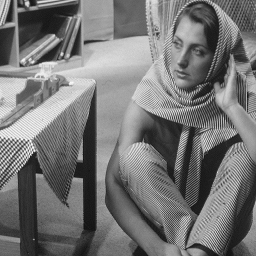
\includegraphics[width=1.5in]{Figure/barbara.png}
\caption{原始图像}
\end{subfigure}
\begin{subfigure}[t]{1.5in}
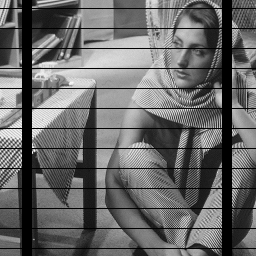
\includegraphics[width=1.5in]{Figure/barbara_mask.png}
\caption{被遮挡的图像}
\end{subfigure}
\begin{subfigure}[t]{1.5in}
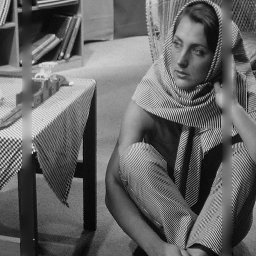
\includegraphics[width=1.5in]{Figure/barbara_out.png}
\caption{恢复的图像}
\end{subfigure}
\caption{Barbara 图像的遮挡和恢复结果}
\label{fig:BarbaraMask}
\end{figure}

尽管如此,我们仍可以借鉴图像修补问题的思想,用于压缩感知问题。我们称图像修补
问题的遮挡矩阵为 $H_1$ ,压缩采样的测量矩阵为 $H_2$。对于图像修补,求解全
变分最小化问题可以恢复原图像,直观地看,这是由于 $H_1$ 的零空间包含被遮挡的
点,优化算法可以自由改变它们的值,以达到减小全变分的目的。同样的,在我们的
压缩感知理论中,鉴于无法确定被遮挡的值,同样应该将这些点加入零空间,使其
可以自由变化。为了达到这一目的,采用矩阵
\begin{equation}
H = H_2 H_1
\end{equation}
作为新的测量矩阵。其中,$H_1$ 的零空间包含所有被遮挡的像素点,赋予了优化算
法足够的自由度,可以通过调整这些点的值尽量降低全变分,使它们不对最终的目标
函数产生较大影响。 $H_2$ 则满足 RIP ,因此其不涉及被遮挡点的子矩阵同样满足
RIP,使得未被遮挡的像素点能够稳定、准确地被恢复。

\section{系统仿真}

测试用例如图 \ref{fig:opttestdata} 所示。图 \ref{fig:opttestdata:in}
是带有栅状电极遮挡的,具有清晰边缘(稀疏梯度)的坏块图像,图
\ref{fig:opttestdata:finger} 是单独提取出的栅电极图层,用于模拟光学成像
确认的栅电极覆盖区域。

\begin{figure}
\centering
\begin{subfigure}[h]{1.5in}
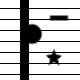
\includegraphics{Figure/testdata/2dsharp_finger.png}
\caption{被遮挡的坏块}
\label{fig:opttestdata:in}
\end{subfigure}
\begin{subfigure}[h]{1.5in}
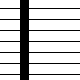
\includegraphics{Figure/testdata/finger.png}
\caption{栅状电极遮挡区域}
\label{fig:opttestdata:finger}
\end{subfigure}
\caption{光学辅助压缩感知缺陷检测测试用例}
\label{fig:opttestdata}
\end{figure}

采用全变分最小化恢复得到的结果如图 \ref{fig:opttv} 所示。可见,将遮挡区域
加入零空间后,只需要 $10\%$ 至 $20\%$ 的采样,即可较好地恢复出坏块。比较
未改进的结果(图 \ref{fig:TVfinger},需要 $50\%$ 采样),可见这一改进对算法
的恢复能力有较大的提升作用。

\begin{figure}
\centering
\begin{subfigure}[h]{1.1in}
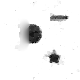
\includegraphics{Figure/TV/opt1.png}
\caption{$M = 0.1N$}
\end{subfigure}
\begin{subfigure}[h]{1.1in}
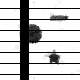
\includegraphics{Figure/TV/opt1f.png}
\caption{叠加栅电极}
\end{subfigure}
\begin{subfigure}[h]{1.1in}
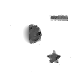
\includegraphics{Figure/TV/opt2.png}
\caption{$M = 0.2N$}
\end{subfigure}
\begin{subfigure}[h]{1.1in}
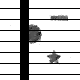
\includegraphics{Figure/TV/opt2f.png}
\caption{叠加栅电极}
\end{subfigure}
\caption{采用光学成像辅助的全变分最小化恢复仿真结果}
\label{fig:opttv}
\end{figure}

此外,$\ell_1$ 范数最小化恢复也可以用完全相同的方法加以改进,只要用
$H_2 H_1$ 作为测量矩阵,即可消除栅电极的
影响。和改进前需要 $50\%$ 测量相比,改进后只需要 $20\%$ 测量即可取得
较好的恢复结果,如图 \ref{fig:optl1} 所示。

\begin{figure}
\centering
\begin{subfigure}[h]{1.1in}
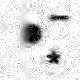
\includegraphics{Figure/L1/opt2.png}
\caption{$M = 0.2N$}
\end{subfigure}
\begin{subfigure}[h]{1.1in}
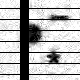
\includegraphics{Figure/L1/opt2f.png}
\caption{叠加栅电极}
\end{subfigure}
\begin{subfigure}[h]{1.1in}
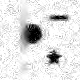
\includegraphics{Figure/L1/opt3.png}
\caption{$M = 0.3N$}
\end{subfigure}
\begin{subfigure}[h]{1.1in}
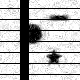
\includegraphics{Figure/L1/opt3f.png}
\caption{叠加栅电极}
\end{subfigure}
\caption{采用光学成像辅助的全变分最小化恢复仿真结果}
\label{fig:optl1}
\end{figure}
